\setcounter{section}{0}
\setlength{\parindent}{0pt}  % niente rientro
\setlength{\parskip}{6pt}  
\section{Il progetto Rinova}
\subsection{Slide pitch}
  % spazio verticale tra paragrafi
\begin{figure}[h!]
    \centering
    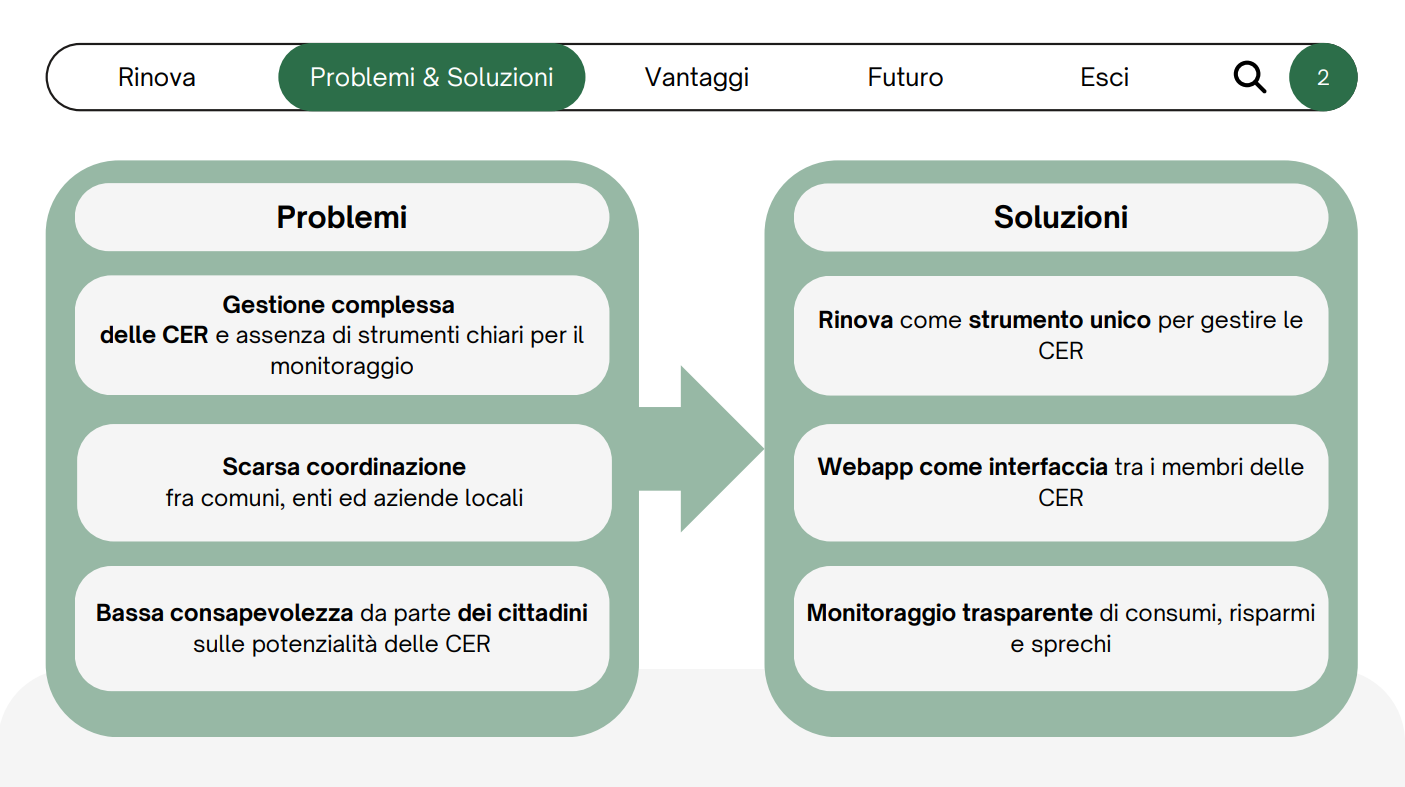
\includegraphics[width=0.3\textwidth]{images/pitch_slide1.png}
    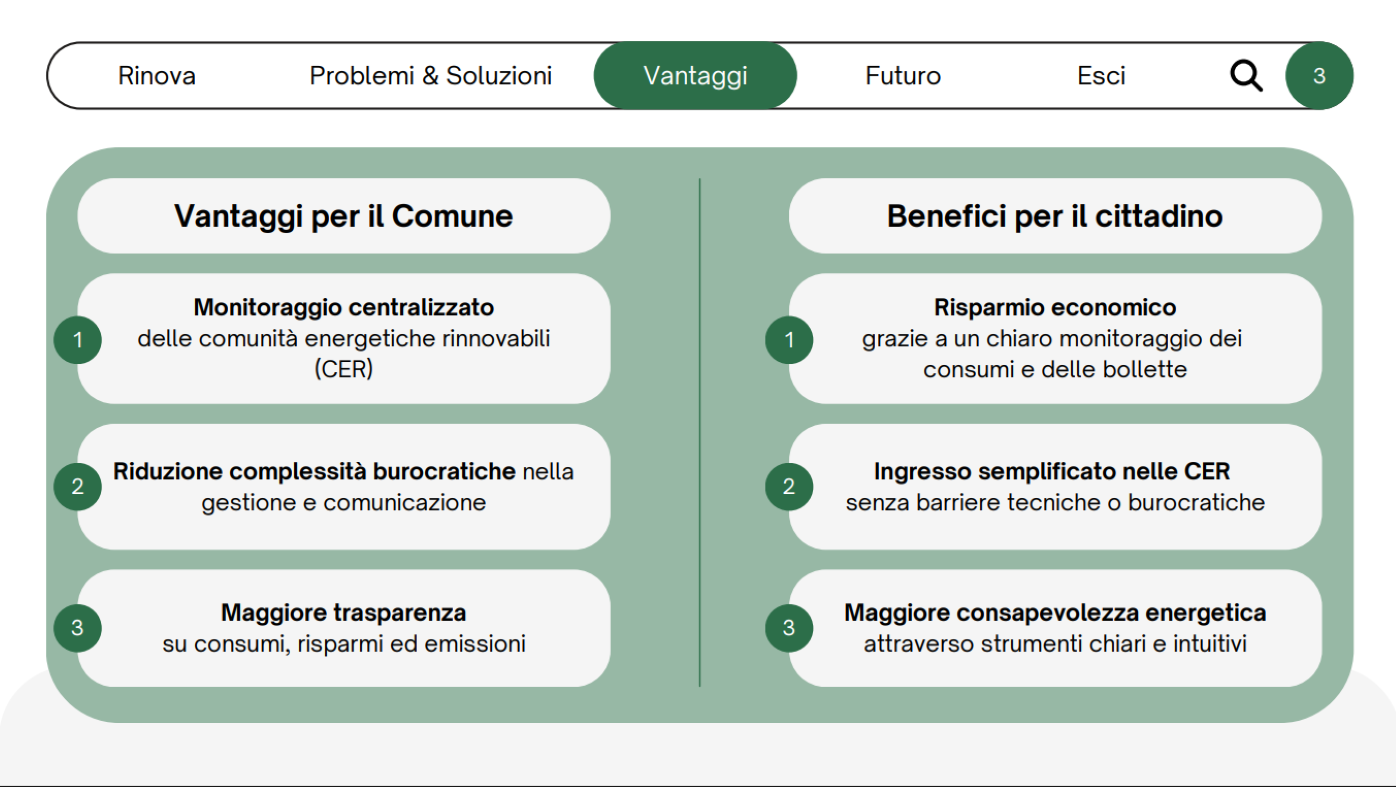
\includegraphics[width=0.3\textwidth]{images/pitch_slide2.png}
    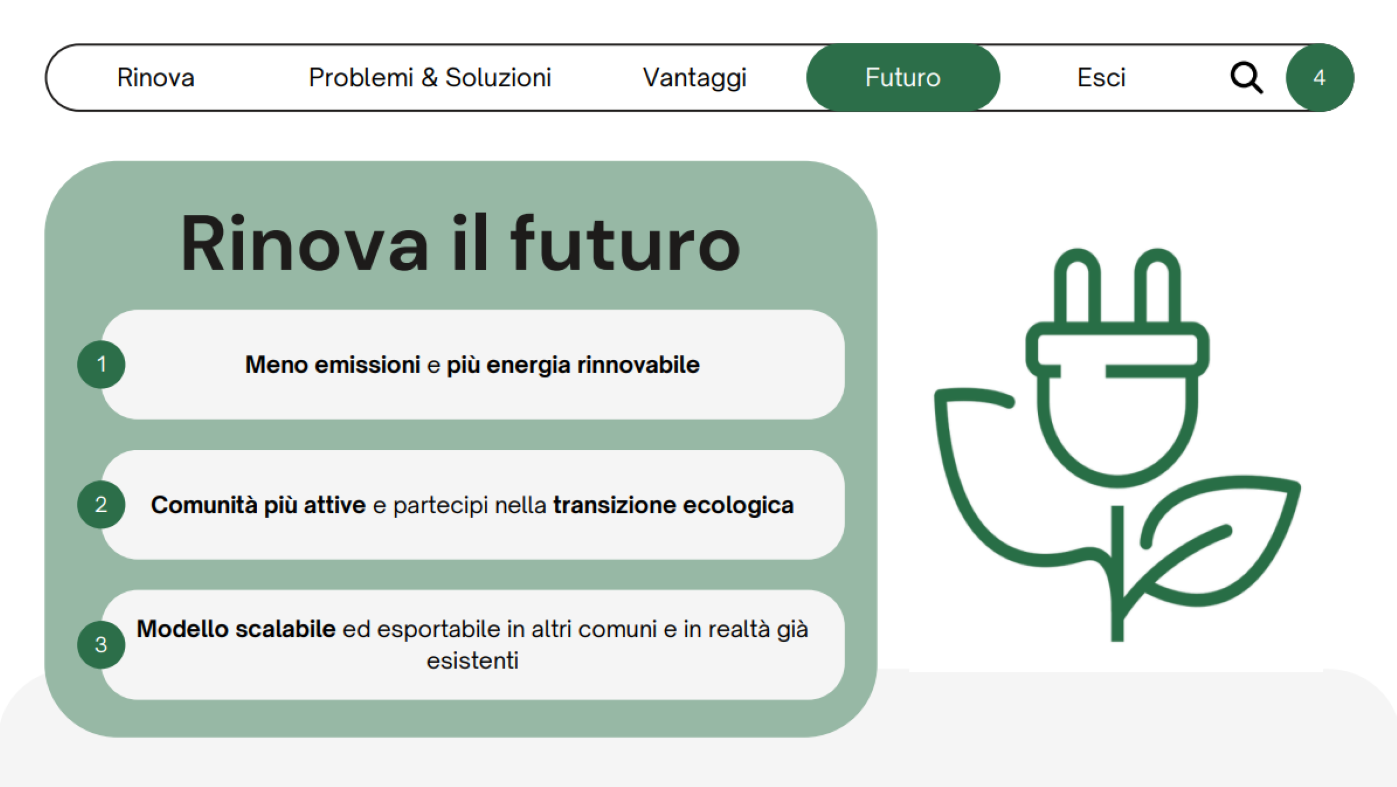
\includegraphics[width=0.3\textwidth]{images/pitch_slide3.png}
    \caption{Slide del pitch di presentazione del progetto Rinova.}
\end{figure}

\subsection{Descrizione del problema}
La crescente necessità di una transizione verso fonti energetiche sostenibili ha portato all’emergere delle Comunità Energetiche Rinnovabili (CER) come strumento strategico per favorire la produzione e la condivisione di energia rinnovabile a livello locale.

Tuttavia, nonostante il loro potenziale, la loro diffusione e sviluppo risultano significativamente ostacolati da alcune problematiche di carattere strutturale e organizzativo.

Ad oggi ancora non esiste un sistema che consenta di gestire e monitorare in modo centralizzato le Comunità Energetiche presenti sul territorio, il che complica notevolmente la raccolta dati, rendendoli frammentati e disorganizzati. Tutto ciò contribuisce al rallentamento della transizione energetica.

L’attuale organizzazione decentralizzata non è l’unica questione da affrontare. Il principale freno alla loro adozione è rappresentato dai costi iniziali elevati e dalla burocrazia complessa. L’indagine condotta a maggio 2025 rileva che il 64\% degli intervistati indica gli alti costi di avvio come ostacolo, seguito dal 46\% che segnala la lentezza delle procedure burocratiche e dal 32\% che lamenta semplicemente di avere “poca informazione” sul tema. Nelle risposte aperte emergono timori concreti quali “tempistiche troppo lunghe”, “incentivi poco chiari” e iter autorizzativi farraginosi. Anche l’analisi Legambiente/Ipsos sottolinea il rischio burocratico: le CER sono viste come grande opportunità, ma “il timore” è che la burocrazia possa ostacolare lo sviluppo e la diffusione di queste iniziative.

C’è poi da sottolineare che i cittadini che hanno risposto a questa intervista rappresentano solo una minoranza rispetto a coloro che di CER non ne hanno nemmeno sentito parlare: un sondaggio Ipsos (Forum QualEnergia 2024) rileva che appena il 14\% della popolazione italiana dichiara di conoscere bene le CER; tra chi già conosce le energie rinnovabili la quota sale al 37\%, ma rimane minoritaria. Analogamente, un’indagine nazionale (maggio 2025) segnala che solo il 25\% del campione conosce pienamente il concetto di CER, un 50\% ne ha solo sentito parlare e il restante 25\% non ne ha proprio idea.

Nonostante ciò, le CER godono di ampio consenso: il 76\% degli intervistati le giudica un’opportunità, ritenendo che possano portare benefici ambientali, economici e sociali. In sintesi, c’è un forte desiderio di cambiamento e interesse verso le Comunità Energetiche Rinnovabili, ma la scarsa informazione sul tema evidenzia la necessità di campagne di sensibilizzazione che rendano consapevoli i cittadini dei benefici ambientali ed economici che potrebbero ottenere attraverso i diversi incentivi presenti all’interno delle CER.

La combinazione di questi fattori crea un ambiente inadatto allo sviluppo delle Comunità Energetiche. La mancanza di centralizzazione, la complessità burocratica e la scarsa consapevolezza da parte dei cittadini contribuiscono a rallentarne la crescita, impedendo di sfruttarne appieno le potenzialità nel favorire la sostenibilità, la riduzione delle emissioni e la partecipazione attiva alla transizione energetica. In tutta Italia siamo ancora solo a 213 CER attive (secondo i dati GSE aggiornati a marzo 2025), un numero esiguo che corrisponde a poco più dell’1\% rispetto all’obiettivo PNRR entro il 2026.

A livello locale anche in Trentino numerose iniziative stanno nascendo ma sono ancora limitate. La Provincia autonoma di Trento ha istituito un elenco ufficiale delle CER (dal 2022) per censirle e monitorarne l’impatto sulla decarbonizzazione.

\subsection{Descrizione della soluzione}
Il progetto Rinova ha come obiettivo la realizzazione di una web app di supporto alle Comunità Energetiche Rinnovabili, ai Comuni e ai cittadini, per semplificare la gestione, favorire la collaborazione e migliorare il monitoraggio dei dati energetici.

Per le CER, Rinova offre una piattaforma dedicata al monitoraggio interno dei consumi, della produzione e dei risparmi, oltre a un’interfaccia già pronta da mettere a disposizione dei propri membri, favorendo trasparenza e partecipazione.

Per il Comune, la web app rappresenta un mezzo centralizzato di controllo e coordinamento, utile per monitorare in tempo reale lo stato delle comunità energetiche presenti sul territorio e per instaurare una comunicazione diretta e continua con gli enti e le cooperative già attive.

Per il cittadino invece, costituisce un punto di accesso semplice e intuitivo alle CER: permette di aderire facilmente alla propria comunità, consultare la documentazione necessaria, richiedere assistenza e monitorare l’andamento energetico personale attraverso un’area riservata dedicata.

Il software Rinova sarà completamente fruibile tramite browser, senza la necessità di installare applicazioni aggiuntive, e sarà progettato per garantire un’esperienza utente intuitiva, accessibile e sicura. Particolare attenzione sarà rivolta alla protezione dei dati personali e alla sicurezza delle informazioni energetiche: la piattaforma sarà conforme al Regolamento Europeo GDPR e alle normative nazionali in materia di privacy, assicurando che tutti i dati degli utenti e delle comunità energetiche siano trattati in modo trasparente, cifrato e protetto.

Il sistema integrerà inoltre funzionalità avanzate per migliorare la comunicazione e l’efficienza: notifiche automatiche su variazioni di consumo o produzione, segnalazioni in tempo reale di eventuali anomalie nei dati e strumenti per facilitare il contatto diretto tra cittadini, enti comunali e gestori delle CER.

\subsection{Vantaggi}
%\subsubsection*{Vantaggi per il Comune}
%\begin{itemize}
 %   \item \textbf{Monitoraggio centralizzato delle Comunità Energetiche Rinnovabili (CER):}  
  %  Rinova offre al Comune un unico strumento digitale per raccogliere, visualizzare e analizzare in tempo reale i dati relativi a tutte le CER presenti sul territorio.  
   % Attraverso una dashboard dedicata, l’amministrazione può monitorare produzione, consumi, adesioni, risparmi economici ed emissioni evitate, ottenendo così una visione completa e aggiornata dell’impatto energetico e ambientale locale.  
    %Questo approccio centralizzato consente di pianificare in modo più efficace le politiche di sostenibilità e di supportare la transizione energetica con dati concreti e verificabili.
    
    %\item \textbf{Riduzione della complessità burocratica nella gestione e comunicazione:}  
    %La piattaforma semplifica i flussi di lavoro tra Comune, enti gestori e cittadini, digitalizzando processi che oggi sono spesso frammentati o manuali.  
    %Rinova riduce il numero di passaggi amministrativi, velocizza la gestione delle adesioni e delle autorizzazioni e migliora la comunicazione diretta con le CER già attive.
    
    %\item \textbf{Maggiore trasparenza su consumi, risparmi ed emissioni:}  
    %Tutti i dati energetici vengono aggregati e resi facilmente consultabili, permettendo al Comune di comunicare in modo chiaro ai cittadini i risultati ottenuti in termini di risparmio economico, energia rinnovabile prodotta e riduzione di CO₂.  
    %La trasparenza favorisce la fiducia e la partecipazione attiva dei cittadini, oltre a rendere più semplice la rendicontazione verso enti superiori e programmi di finanziamento pubblici.
%\end{itemize}
\subsubsection*{Benefici per le Comunità Energetiche Rinnovabili (CER)}
\begin{itemize}
    \item \textbf{Interfaccia tra CER e membri:}  
    Rinova si propone come piattaforma digitale di riferimento per la comunicazione tra le comunità energetiche e i propri membri.  
    Seppur per obbligo di legge ogni CER debba disporre di un proprio sito web, non è raro trovare siti non aggiornati o non più attivi. Le CER potranno quindi utilizzare la web app come spazio dedicato, eliminando la necessità di sviluppare un sito web autonomo e riducendo così costi di gestione, manutenzione e sviluppo.
    
    \item \textbf{Strumento per il monitoraggio dei dati interni:}  
    Rinova fornisce alle CER una dashboard completa per il controllo dei dati operativi: consumi, produzione energetica, adesione di nuovi membri, energia condivisa e risparmi ottenuti.  
    Questi dati, visualizzati in tempo reale, consentono di valutare l’efficienza della comunità, migliorare la gestione e rendicontare con precisione i risultati sia verso i membri che verso gli enti pubblici.
\end{itemize}

\subsubsection*{Benefici per il cittadino}
\begin{itemize}
    \item \textbf{Risparmio economico grazie a un chiaro monitoraggio dei consumi e delle bollette:}  
    Rinova consente ai cittadini di visualizzare in modo semplice e immediato i propri consumi energetici, i costi associati e i risparmi ottenuti grazie alla partecipazione alla comunità energetica.  
    Attraverso grafici e indicatori intuitivi, l’utente può comprendere meglio l’andamento dei propri consumi e ottimizzare l’uso dell’energia.
    
    \begin{comment}    
    \item \textbf{Ingresso semplificato nelle CER, senza barriere tecniche o burocratiche:}  
    Rinova offre un sistema di adesione guidato e digitalizzato, che consente al cittadino di entrare nella propria comunità energetica in modo semplice e autonomo.  
    Attraverso la piattaforma è possibile accedere alle informazioni sulle CER attive, scaricare la documentazione necessaria e seguire una procedura di iscrizione passo-passo.  
    L’obiettivo è eliminare le barriere di accesso legate alla burocrazia e rendere la partecipazione alle CER alla portata di tutti.
    \end{comment}
    
    \item \textbf{Maggiore consapevolezza energetica attraverso strumenti chiari e intuitivi:}  
    L’area personale del cittadino fornisce una panoramica completa sul proprio contributo alla comunità: energia condivisa, emissioni di CO₂ evitate e risparmi generati.  
    Queste informazioni permettono all’utente di percepire concretamente l’impatto positivo delle proprie scelte, rafforzando la cultura della sostenibilità e la partecipazione attiva alla transizione energetica.
\end{itemize}

\subsection{Limitazioni e problemi}
\begin{itemize}
    \item \textbf{Frequenti e repentini cambiamenti delle normative:}  
    L’ambito delle CER è fortemente regolamentato da normative burocratiche soggette a continui cambiamenti. È quindi necessario prevedere aggiornamenti e manutenzioni costanti per adeguarsi alle nuove leggi, con possibili costi aggiuntivi e interruzioni temporanee del servizio.
    
    \item \textbf{Necessaria la collaborazione di numerose CER:}  
    Per suscitare interesse da parte dei Comuni è necessaria una grande mole di dati, ottenibili solo grazie alla collaborazione di numerose comunità. Uno dei principali servizi di Rinova è quindi fortemente influenzato dal numero di enti che decidono di aderire.
    
    \item \textbf{Sicurezza dei dati:}  
    Nonostante la particolare attenzione alla protezione dei dati personali e alla sicurezza delle informazioni energetiche, il rischio di una violazione informatica con possibile furto di dati sensibili rimane presente.
    
    \item \textbf{Necessaria connessione a Internet:}  
    Poiché il compito principale della piattaforma è raccogliere dati su produzione e consumi, è richiesta una connessione Internet stabile e persistente.
    
    \item \textbf{Diffusione dell’applicazione proporzionale allo sviluppo delle CER:}  
    Rinova è rivolta a una fascia di utenza specifica: membri e gestori di comunità energetiche. La crescita della piattaforma dipende quindi dallo sviluppo delle CER sul territorio e dalla creazione di nuove realtà.
    
    \item \textbf{Dipendenza dai dati raccolti dalle CER:}  
    Poiché l’applicazione elabora i dati forniti dalle Comunità Energetiche associate, la qualità delle informazioni dipende strettamente dalle metodologie e dagli strumenti adottati dalle singole comunità. Eventuali problemi o guasti si ripercuotono quindi sui servizi offerti da Rinova.
\end{itemize}
